% Options for packages loaded elsewhere
\PassOptionsToPackage{unicode}{hyperref}
\PassOptionsToPackage{hyphens}{url}
%
\documentclass[
  ignorenonframetext,
]{beamer}
\usepackage{pgfpages}
\setbeamertemplate{caption}[numbered]
\setbeamertemplate{caption label separator}{: }
\setbeamercolor{caption name}{fg=normal text.fg}
\beamertemplatenavigationsymbolsempty
% Prevent slide breaks in the middle of a paragraph
\widowpenalties 1 10000
\raggedbottom
\setbeamertemplate{part page}{
  \centering
  \begin{beamercolorbox}[sep=16pt,center]{part title}
    \usebeamerfont{part title}\insertpart\par
  \end{beamercolorbox}
}
\setbeamertemplate{section page}{
  \centering
  \begin{beamercolorbox}[sep=12pt,center]{part title}
    \usebeamerfont{section title}\insertsection\par
  \end{beamercolorbox}
}
\setbeamertemplate{subsection page}{
  \centering
  \begin{beamercolorbox}[sep=8pt,center]{part title}
    \usebeamerfont{subsection title}\insertsubsection\par
  \end{beamercolorbox}
}
\AtBeginPart{
  \frame{\partpage}
}
\AtBeginSection{
  \ifbibliography
  \else
    \frame{\sectionpage}
  \fi
}
\AtBeginSubsection{
  \frame{\subsectionpage}
}
\usepackage{amsmath,amssymb}
\usepackage{lmodern}
\usepackage{iftex}
\ifPDFTeX
  \usepackage[T1]{fontenc}
  \usepackage[utf8]{inputenc}
  \usepackage{textcomp} % provide euro and other symbols
\else % if luatex or xetex
  \usepackage{unicode-math}
  \defaultfontfeatures{Scale=MatchLowercase}
  \defaultfontfeatures[\rmfamily]{Ligatures=TeX,Scale=1}
\fi
\usetheme[]{Ilmenau}
% Use upquote if available, for straight quotes in verbatim environments
\IfFileExists{upquote.sty}{\usepackage{upquote}}{}
\IfFileExists{microtype.sty}{% use microtype if available
  \usepackage[]{microtype}
  \UseMicrotypeSet[protrusion]{basicmath} % disable protrusion for tt fonts
}{}
\makeatletter
\@ifundefined{KOMAClassName}{% if non-KOMA class
  \IfFileExists{parskip.sty}{%
    \usepackage{parskip}
  }{% else
    \setlength{\parindent}{0pt}
    \setlength{\parskip}{6pt plus 2pt minus 1pt}}
}{% if KOMA class
  \KOMAoptions{parskip=half}}
\makeatother
\usepackage{xcolor}
\newif\ifbibliography
\usepackage{color}
\usepackage{fancyvrb}
\newcommand{\VerbBar}{|}
\newcommand{\VERB}{\Verb[commandchars=\\\{\}]}
\DefineVerbatimEnvironment{Highlighting}{Verbatim}{commandchars=\\\{\}}
% Add ',fontsize=\small' for more characters per line
\usepackage{framed}
\definecolor{shadecolor}{RGB}{248,248,248}
\newenvironment{Shaded}{\begin{snugshade}}{\end{snugshade}}
\newcommand{\AlertTok}[1]{\textcolor[rgb]{0.94,0.16,0.16}{#1}}
\newcommand{\AnnotationTok}[1]{\textcolor[rgb]{0.56,0.35,0.01}{\textbf{\textit{#1}}}}
\newcommand{\AttributeTok}[1]{\textcolor[rgb]{0.77,0.63,0.00}{#1}}
\newcommand{\BaseNTok}[1]{\textcolor[rgb]{0.00,0.00,0.81}{#1}}
\newcommand{\BuiltInTok}[1]{#1}
\newcommand{\CharTok}[1]{\textcolor[rgb]{0.31,0.60,0.02}{#1}}
\newcommand{\CommentTok}[1]{\textcolor[rgb]{0.56,0.35,0.01}{\textit{#1}}}
\newcommand{\CommentVarTok}[1]{\textcolor[rgb]{0.56,0.35,0.01}{\textbf{\textit{#1}}}}
\newcommand{\ConstantTok}[1]{\textcolor[rgb]{0.00,0.00,0.00}{#1}}
\newcommand{\ControlFlowTok}[1]{\textcolor[rgb]{0.13,0.29,0.53}{\textbf{#1}}}
\newcommand{\DataTypeTok}[1]{\textcolor[rgb]{0.13,0.29,0.53}{#1}}
\newcommand{\DecValTok}[1]{\textcolor[rgb]{0.00,0.00,0.81}{#1}}
\newcommand{\DocumentationTok}[1]{\textcolor[rgb]{0.56,0.35,0.01}{\textbf{\textit{#1}}}}
\newcommand{\ErrorTok}[1]{\textcolor[rgb]{0.64,0.00,0.00}{\textbf{#1}}}
\newcommand{\ExtensionTok}[1]{#1}
\newcommand{\FloatTok}[1]{\textcolor[rgb]{0.00,0.00,0.81}{#1}}
\newcommand{\FunctionTok}[1]{\textcolor[rgb]{0.00,0.00,0.00}{#1}}
\newcommand{\ImportTok}[1]{#1}
\newcommand{\InformationTok}[1]{\textcolor[rgb]{0.56,0.35,0.01}{\textbf{\textit{#1}}}}
\newcommand{\KeywordTok}[1]{\textcolor[rgb]{0.13,0.29,0.53}{\textbf{#1}}}
\newcommand{\NormalTok}[1]{#1}
\newcommand{\OperatorTok}[1]{\textcolor[rgb]{0.81,0.36,0.00}{\textbf{#1}}}
\newcommand{\OtherTok}[1]{\textcolor[rgb]{0.56,0.35,0.01}{#1}}
\newcommand{\PreprocessorTok}[1]{\textcolor[rgb]{0.56,0.35,0.01}{\textit{#1}}}
\newcommand{\RegionMarkerTok}[1]{#1}
\newcommand{\SpecialCharTok}[1]{\textcolor[rgb]{0.00,0.00,0.00}{#1}}
\newcommand{\SpecialStringTok}[1]{\textcolor[rgb]{0.31,0.60,0.02}{#1}}
\newcommand{\StringTok}[1]{\textcolor[rgb]{0.31,0.60,0.02}{#1}}
\newcommand{\VariableTok}[1]{\textcolor[rgb]{0.00,0.00,0.00}{#1}}
\newcommand{\VerbatimStringTok}[1]{\textcolor[rgb]{0.31,0.60,0.02}{#1}}
\newcommand{\WarningTok}[1]{\textcolor[rgb]{0.56,0.35,0.01}{\textbf{\textit{#1}}}}
\usepackage{graphicx}
\makeatletter
\def\maxwidth{\ifdim\Gin@nat@width>\linewidth\linewidth\else\Gin@nat@width\fi}
\def\maxheight{\ifdim\Gin@nat@height>\textheight\textheight\else\Gin@nat@height\fi}
\makeatother
% Scale images if necessary, so that they will not overflow the page
% margins by default, and it is still possible to overwrite the defaults
% using explicit options in \includegraphics[width, height, ...]{}
\setkeys{Gin}{width=\maxwidth,height=\maxheight,keepaspectratio}
% Set default figure placement to htbp
\makeatletter
\def\fps@figure{htbp}
\makeatother
\setlength{\emergencystretch}{3em} % prevent overfull lines
\providecommand{\tightlist}{%
  \setlength{\itemsep}{0pt}\setlength{\parskip}{0pt}}
\setcounter{secnumdepth}{-\maxdimen} % remove section numbering
\setbeamertemplate{navigation symbols}{}
\setbeamertemplate{footline}[page number]
\ifLuaTeX
  \usepackage{selnolig}  % disable illegal ligatures
\fi
\IfFileExists{bookmark.sty}{\usepackage{bookmark}}{\usepackage{hyperref}}
\IfFileExists{xurl.sty}{\usepackage{xurl}}{} % add URL line breaks if available
\urlstyle{same} % disable monospaced font for URLs
\hypersetup{
  pdftitle={Multivariate Analysis Lecture 2: MatrixOperations},
  hidelinks,
  pdfcreator={LaTeX via pandoc}}

\title{Multivariate Analysis Lecture 2: MatrixOperations}
\author{Zhaoxia Yu\\
Professor, Department of Statistics}
\date{2023-04-06}

\begin{document}
\frame{\titlepage}

\hypertarget{matrix-multiplication}{%
\subsection{Matrix Multiplication}\label{matrix-multiplication}}

\begin{frame}{Definition of Matrix Multiplication}
\protect\hypertarget{definition-of-matrix-multiplication}{}
\begin{itemize}
\tightlist
\item
  Consider matrix \(A_{m\times n}\) and matrix \(B_{n\times p}\).
\item
  How does \(AB\) look like?
\item
  \(AB\) has \(m\) rows and \(p\) columns
\item
  What is the value in the \(i\)th row and \(j\)th column of \(AB\)? We
  often denote it as the \((i,j)\)th element/entry of \(AB\):
  \[\left(AB\right)_{i,j}=\sum_{k=1}^n a_{ik}b_{kj}\]
\end{itemize}
\end{frame}

\begin{frame}{Definition of Matrix Multiplication}
\protect\hypertarget{definition-of-matrix-multiplication-1}{}
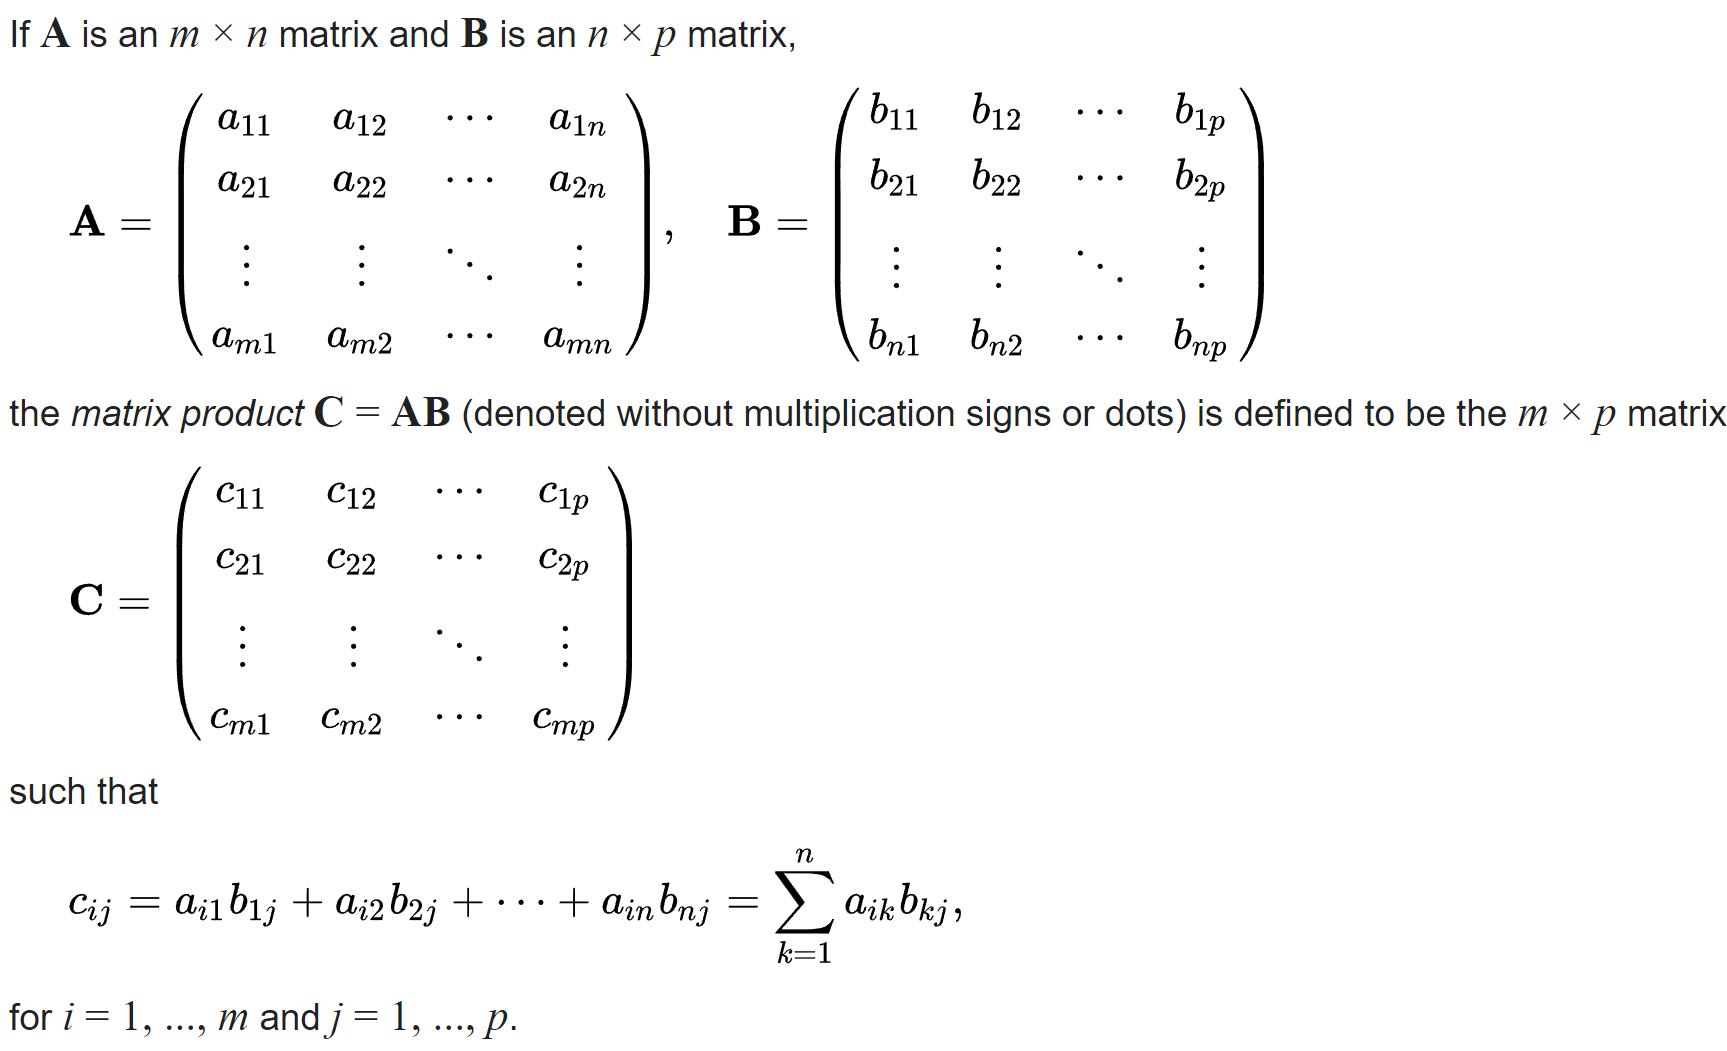
\includegraphics[width=0.9\linewidth]{img/MatrixMultiplicationWiki}
\end{frame}

\begin{frame}{Matrix Multiplication}
\protect\hypertarget{matrix-multiplication-1}{}
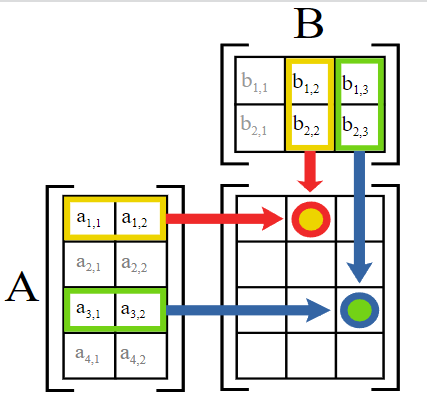
\includegraphics[width=0.5\linewidth]{img/MatrixMultiplication}
\end{frame}

\begin{frame}{Conformable Matrices}
\protect\hypertarget{conformable-matrices}{}
\begin{itemize}
\tightlist
\item
  Conformability refers to whether two matrices can be multiplied.\\
\item
  Two matrices can be multiplied if they are
  \textcolor{red}{conformable}.\\
\item
  E.g., if \(dim(A)=n\times 10, dim(B)=10\times p\), then \(A\) and
  \(B\) are conformable because we can compute \(AB\).
\item
  Note: If \(A\) and \(B\) is conformable for calculating \(AB\), it
  doesn't guarantee that they are also conformable for calculating
  \(BA\).
\item
  conformable for multiplication, then the operation is not defined.
\end{itemize}
\end{frame}

\hypertarget{the-iris-data}{%
\subsection{The Iris Data}\label{the-iris-data}}

\begin{frame}{Iris data}
\protect\hypertarget{iris-data}{}
\begin{itemize}
\tightlist
\item
  Three species of iris flowers: setosa, versicolor, and virginica
\item
  Four features: sepal length, sepal width, petal length, and petal
  width
\end{itemize}

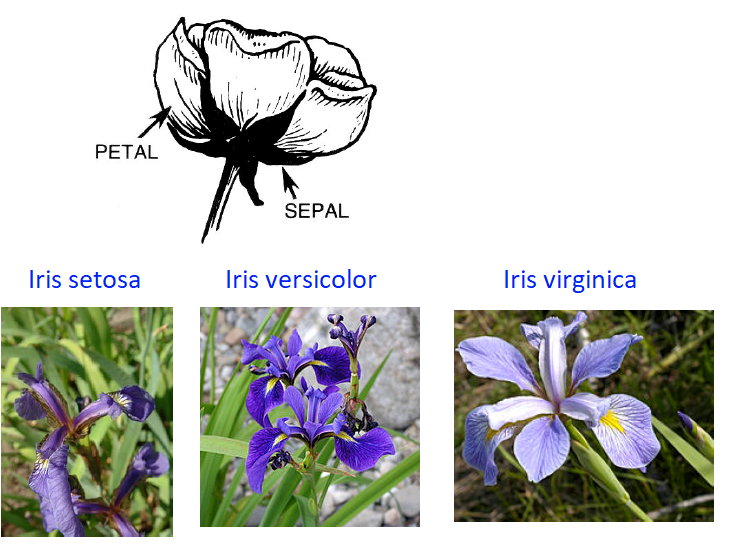
\includegraphics[width=0.6\linewidth]{img/iris}
\end{frame}

\begin{frame}{Introduction}
\protect\hypertarget{introduction}{}
\begin{itemize}
\tightlist
\item
  The iris dataset is a widely used dataset to illustrate various
  methods, algorithms, and problems.
\item
  Iris dataset serves as an excellent example of how data can be used to
  gain insights into different fields.
\item
  It is available in many places

  \begin{itemize}
  \tightlist
  \item
    It is available from UCI Machine Learning Repository.\\
  \item
    It is also included as a built-in data set in R. Use ``data()'' to
    see the list of built-in data sets.
  \item
    Wikipedia has a page for the dataset.\\
  \end{itemize}
\item
  Its simplicity and easy availability have made it a widely used
  dataset for educational and research purposes.
\end{itemize}
\end{frame}

\begin{frame}{History}
\protect\hypertarget{history}{}
\begin{itemize}
\tightlist
\item
  The iris dataset has a rich history and has been used in many
  different areas of research
\item
  It was first introduced by Ronald Fisher in 1936.
\item
  The dataset contains measurements of four features of three species of
  iris flowers.
\item
  Fisher used the iris dataset as an example of discriminant analysis
\end{itemize}
\end{frame}

\begin{frame}{Iris data}
\protect\hypertarget{iris-data-1}{}
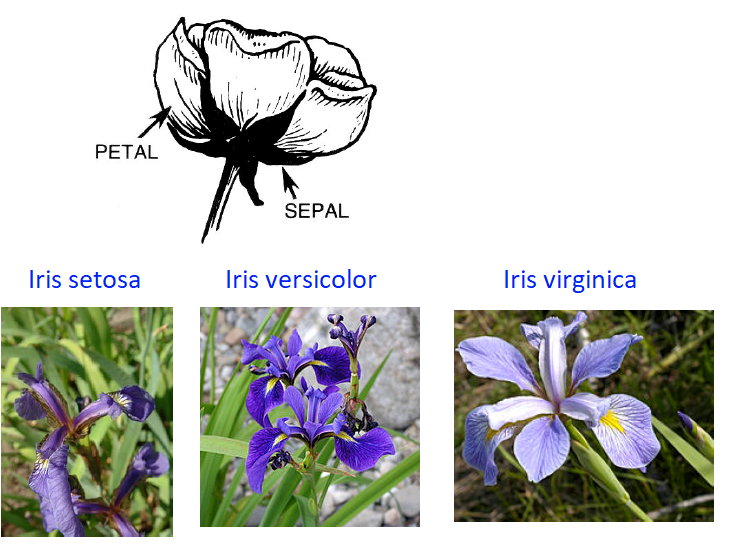
\includegraphics[width=0.7\linewidth]{img/iris}
\end{frame}

\begin{frame}[fragile]{Iris data in R}
\protect\hypertarget{iris-data-in-r}{}
\begin{itemize}
\tightlist
\item
  The iris data is stored in two different formats:

  \begin{itemize}
  \tightlist
  \item
    as a 3D array: iris3
  \item
    as a long matrix: iris
  \end{itemize}
\end{itemize}

\begin{Shaded}
\begin{Highlighting}[]
\CommentTok{\#?iris}
\FunctionTok{dim}\NormalTok{(iris3)}
\end{Highlighting}
\end{Shaded}

\begin{verbatim}
## [1] 50  4  3
\end{verbatim}

\begin{Shaded}
\begin{Highlighting}[]
\FunctionTok{dim}\NormalTok{(iris)}
\end{Highlighting}
\end{Shaded}

\begin{verbatim}
## [1] 150   5
\end{verbatim}
\end{frame}

\begin{frame}[fragile]{Iris data in R}
\protect\hypertarget{iris-data-in-r-1}{}
\begin{Shaded}
\begin{Highlighting}[]
\FunctionTok{dimnames}\NormalTok{(iris3)}
\end{Highlighting}
\end{Shaded}

\begin{verbatim}
## [[1]]
## NULL
## 
## [[2]]
## [1] "Sepal L." "Sepal W." "Petal L." "Petal W."
## 
## [[3]]
## [1] "Setosa"     "Versicolor" "Virginica"
\end{verbatim}

\begin{Shaded}
\begin{Highlighting}[]
\FunctionTok{names}\NormalTok{(iris)}
\end{Highlighting}
\end{Shaded}

\begin{verbatim}
## [1] "Sepal.Length" "Sepal.Width"  "Petal.Length" "Petal.Width"  "Species"
\end{verbatim}
\end{frame}

\begin{frame}[fragile]{Iris data in R}
\protect\hypertarget{iris-data-in-r-2}{}
\begin{Shaded}
\begin{Highlighting}[]
\CommentTok{\#the attributes is a useful function to understand data}
\FunctionTok{attributes}\NormalTok{(iris3)}
\end{Highlighting}
\end{Shaded}

\begin{verbatim}
## $dim
## [1] 50  4  3
## 
## $dimnames
## $dimnames[[1]]
## NULL
## 
## $dimnames[[2]]
## [1] "Sepal L." "Sepal W." "Petal L." "Petal W."
## 
## $dimnames[[3]]
## [1] "Setosa"     "Versicolor" "Virginica"
\end{verbatim}
\end{frame}

\begin{frame}[fragile]{Iris data in R}
\protect\hypertarget{iris-data-in-r-3}{}
\begin{Shaded}
\begin{Highlighting}[]
\CommentTok{\#the attributes is a useful function to understand data}
\FunctionTok{attributes}\NormalTok{(iris)}
\end{Highlighting}
\end{Shaded}

\begin{verbatim}
## $names
## [1] "Sepal.Length" "Sepal.Width"  "Petal.Length" "Petal.Width"  "Species"     
## 
## $class
## [1] "data.frame"
## 
## $row.names
##   [1]   1   2   3   4   5   6   7   8   9  10  11  12  13  14  15  16  17  18
##  [19]  19  20  21  22  23  24  25  26  27  28  29  30  31  32  33  34  35  36
##  [37]  37  38  39  40  41  42  43  44  45  46  47  48  49  50  51  52  53  54
##  [55]  55  56  57  58  59  60  61  62  63  64  65  66  67  68  69  70  71  72
##  [73]  73  74  75  76  77  78  79  80  81  82  83  84  85  86  87  88  89  90
##  [91]  91  92  93  94  95  96  97  98  99 100 101 102 103 104 105 106 107 108
## [109] 109 110 111 112 113 114 115 116 117 118 119 120 121 122 123 124 125 126
## [127] 127 128 129 130 131 132 133 134 135 136 137 138 139 140 141 142 143 144
## [145] 145 146 147 148 149 150
\end{verbatim}
\end{frame}

\begin{frame}[fragile]{Heatmap of the Iris Data}
\protect\hypertarget{heatmap-of-the-iris-data}{}
\begin{Shaded}
\begin{Highlighting}[]
\NormalTok{Y}\OtherTok{=}\FunctionTok{as.matrix}\NormalTok{(iris[, }\DecValTok{1}\SpecialCharTok{:}\DecValTok{4}\NormalTok{])}
\FunctionTok{rownames}\NormalTok{(Y)}\OtherTok{=}\NormalTok{iris[,}\DecValTok{5}\NormalTok{]}
\FunctionTok{heatmap}\NormalTok{(Y[}\DecValTok{150}\SpecialCharTok{:}\DecValTok{1}\NormalTok{, ],}\AttributeTok{col=}\FunctionTok{rainbow}\NormalTok{(}\DecValTok{12}\NormalTok{),}\AttributeTok{Rowv=}\ConstantTok{NA}\NormalTok{, }\AttributeTok{Colv=}\ConstantTok{NA}\NormalTok{)}
\end{Highlighting}
\end{Shaded}
\end{frame}

\begin{frame}{Heatmap of the Iris Data}
\protect\hypertarget{heatmap-of-the-iris-data-1}{}
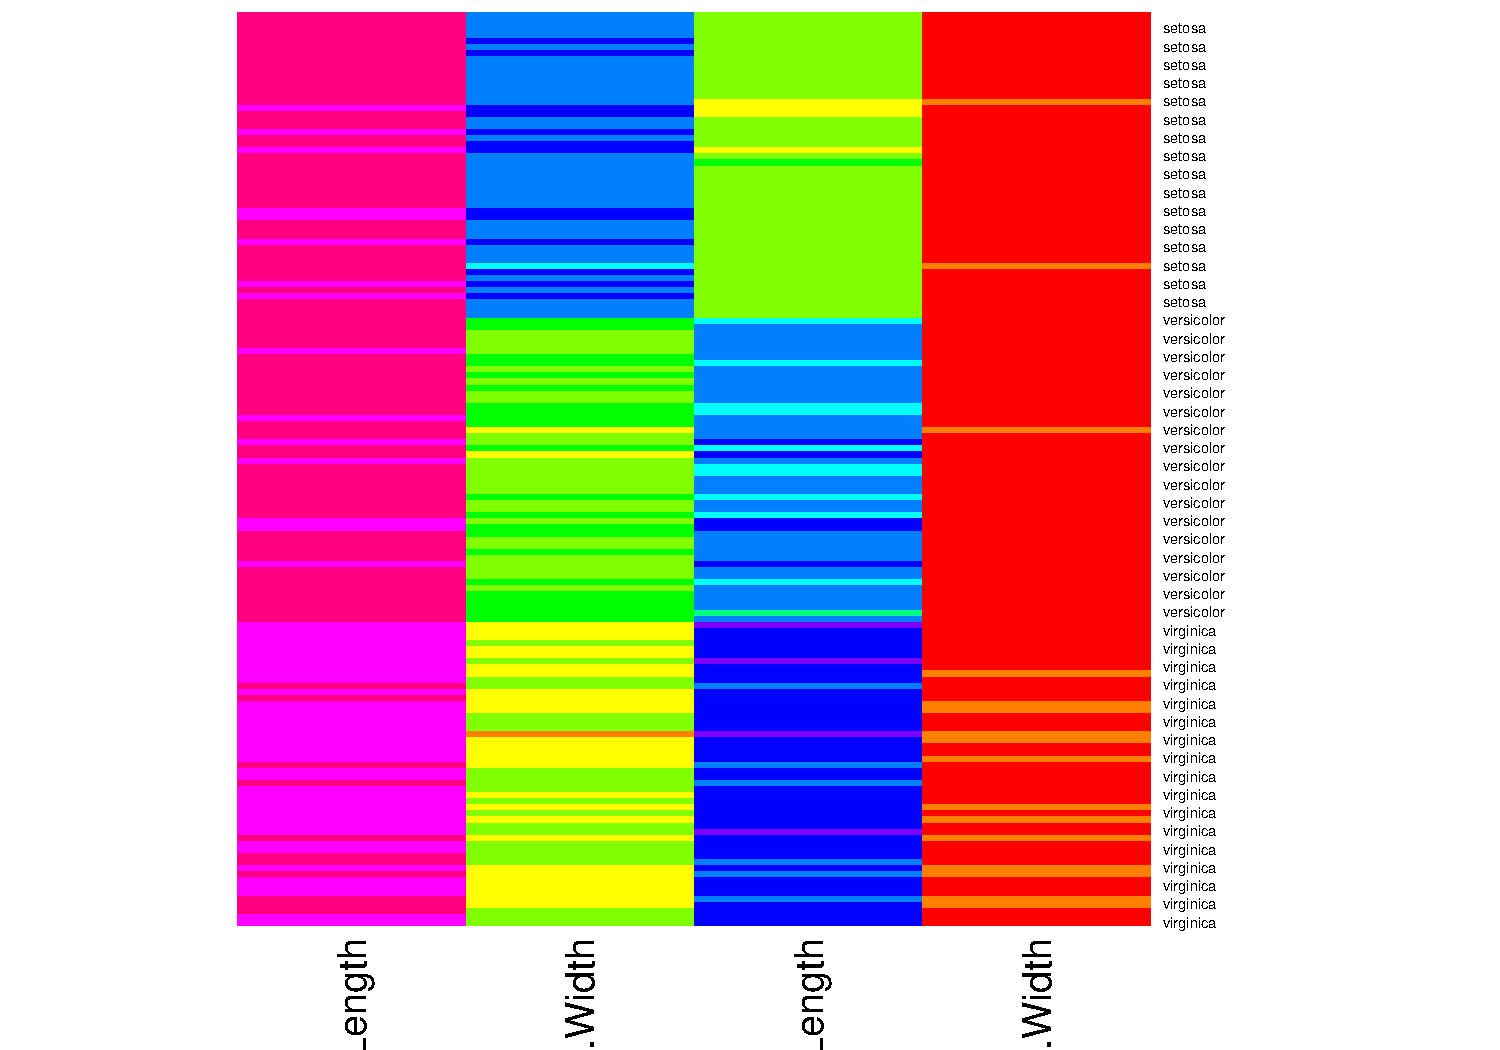
\includegraphics[width=0.6\linewidth]{Lecture02_MatrixOperations_files/figure-beamer/unnamed-chunk-10-1}
\end{frame}

\begin{frame}[fragile]{Left multiply a matrix to Y: Example 1}
\protect\hypertarget{left-multiply-a-matrix-to-y-example-1}{}
\begin{itemize}
\tightlist
\item
  Consider \[A=\frac{1}{150}\mathbf{1}_{1\times 150},\] i.e.,
  \[A_{1\times 150}=(\frac{1}{150}, \cdots, \frac{1}{150})\]
\item
  What is \(AY\)?
\item
  In R, the correct syntax for matrix multiplication is
\end{itemize}

\begin{verbatim}
%*%
\end{verbatim}
\end{frame}

\begin{frame}[fragile]{Left multiply a matrix to Y: Example 1}
\protect\hypertarget{left-multiply-a-matrix-to-y-example-1-1}{}
\begin{Shaded}
\begin{Highlighting}[]
\NormalTok{A}\OtherTok{=}\FunctionTok{matrix}\NormalTok{(}\DecValTok{1}\SpecialCharTok{/}\DecValTok{150}\NormalTok{, }\DecValTok{1}\NormalTok{, }\DecValTok{150}\NormalTok{)}
\NormalTok{A}\SpecialCharTok{\%*\%}\NormalTok{Y}
\end{Highlighting}
\end{Shaded}

\begin{verbatim}
##      Sepal.Length Sepal.Width Petal.Length Petal.Width
## [1,]     5.843333    3.057333        3.758    1.199333
\end{verbatim}

\begin{Shaded}
\begin{Highlighting}[]
\FunctionTok{dim}\NormalTok{(A}\SpecialCharTok{\%*\%}\NormalTok{Y)}
\end{Highlighting}
\end{Shaded}

\begin{verbatim}
## [1] 1 4
\end{verbatim}
\end{frame}

\begin{frame}[fragile]{Left multiply a matrix to Y: Example 1}
\protect\hypertarget{left-multiply-a-matrix-to-y-example-1-2}{}
\begin{itemize}
\tightlist
\item
  Let's check the results
\end{itemize}

\begin{Shaded}
\begin{Highlighting}[]
\NormalTok{A}\SpecialCharTok{\%*\%}\NormalTok{Y}
\end{Highlighting}
\end{Shaded}

\begin{verbatim}
##      Sepal.Length Sepal.Width Petal.Length Petal.Width
## [1,]     5.843333    3.057333        3.758    1.199333
\end{verbatim}

\begin{Shaded}
\begin{Highlighting}[]
\FunctionTok{colMeans}\NormalTok{(Y)}
\end{Highlighting}
\end{Shaded}

\begin{verbatim}
## Sepal.Length  Sepal.Width Petal.Length  Petal.Width 
##     5.843333     3.057333     3.758000     1.199333
\end{verbatim}
\end{frame}

\begin{frame}{Left multiply a matrix to Y: Example 2}
\protect\hypertarget{left-multiply-a-matrix-to-y-example-2}{}
\begin{itemize}
\item
  Let \[B=\frac{1}{50}\begin{pmatrix}
  \mathbf 1_{1\times 50} & \mathbf 1_{1\times 50} & \mathbf 0_{1\times 50}\\
  \mathbf 1_{1\times 50} & \mathbf 0_{1\times 50} & -\mathbf 1_{1\times 50} \\
  \mathbf 0_{1\times 50} & \mathbf 1_{1\times 50} & -\mathbf 1_{1\times 50} \\
  \end{pmatrix}\] i.e., \[B=\begin{pmatrix}
  \frac{1}{50}& \cdots& \frac{1}{50}&
  -\frac{1}{50}& \cdots& -\frac{1}{50}&
  0 & \cdots & 0\\
  \frac{1}{50}& \cdots& \frac{1}{50}&
  0 & \cdots & 0 &
  -\frac{1}{50}& \cdots& -\frac{1}{50}&\\
  0 & \cdots & 0 &
  \frac{1}{50}& \cdots& \frac{1}{50}&
  -\frac{1}{50}& \cdots& -\frac{1}{50}&
  \end{pmatrix}\]
\item
  What does \(BY\) give us?
\end{itemize}
\end{frame}

\begin{frame}[fragile]{Left multiply a matrix to Y: example2}
\protect\hypertarget{left-multiply-a-matrix-to-y-example2}{}
\begin{itemize}
\tightlist
\item
  \(BY\) gives the pairwise difference in group means for each feature
\end{itemize}

\begin{Shaded}
\begin{Highlighting}[]
\NormalTok{B}\OtherTok{=}\DecValTok{1}\SpecialCharTok{/}\DecValTok{50}\SpecialCharTok{*}\FunctionTok{rbind}\NormalTok{(}
  \FunctionTok{rep}\NormalTok{(}\FunctionTok{c}\NormalTok{(}\DecValTok{1}\NormalTok{,}\SpecialCharTok{{-}}\DecValTok{1}\NormalTok{, }\DecValTok{0}\NormalTok{), }\AttributeTok{each=}\DecValTok{50}\NormalTok{), }
  \FunctionTok{rep}\NormalTok{(}\FunctionTok{c}\NormalTok{(}\DecValTok{1}\NormalTok{, }\DecValTok{0}\NormalTok{,}\SpecialCharTok{{-}}\DecValTok{1}\NormalTok{), }\AttributeTok{each=}\DecValTok{50}\NormalTok{), }
  \FunctionTok{rep}\NormalTok{(}\FunctionTok{c}\NormalTok{(}\DecValTok{0}\NormalTok{, }\DecValTok{1}\NormalTok{,}\SpecialCharTok{{-}}\DecValTok{1}\NormalTok{), }\AttributeTok{each=}\DecValTok{50}\NormalTok{))}
\NormalTok{B}\SpecialCharTok{\%*\%}\NormalTok{Y}
\end{Highlighting}
\end{Shaded}

\begin{verbatim}
##      Sepal.Length Sepal.Width Petal.Length Petal.Width
## [1,]       -0.930       0.658       -2.798       -1.08
## [2,]       -1.582       0.454       -4.090       -1.78
## [3,]       -0.652      -0.204       -1.292       -0.70
\end{verbatim}
\end{frame}

\begin{frame}[fragile]{Left multiply a matrix to Y: example2}
\protect\hypertarget{left-multiply-a-matrix-to-y-example2-1}{}
\begin{itemize}
\tightlist
\item
  Let's check results
\end{itemize}

\begin{Shaded}
\begin{Highlighting}[]
\CommentTok{\#colMeans(iris[iris$Species=="setosa",1:4])}
\FunctionTok{colMeans}\NormalTok{(Y[}\DecValTok{1}\SpecialCharTok{:}\DecValTok{50}\NormalTok{,])}
\end{Highlighting}
\end{Shaded}

\begin{verbatim}
## Sepal.Length  Sepal.Width Petal.Length  Petal.Width 
##        5.006        3.428        1.462        0.246
\end{verbatim}

\begin{Shaded}
\begin{Highlighting}[]
\FunctionTok{colMeans}\NormalTok{(Y[}\DecValTok{51}\SpecialCharTok{:}\DecValTok{100}\NormalTok{,])}
\end{Highlighting}
\end{Shaded}

\begin{verbatim}
## Sepal.Length  Sepal.Width Petal.Length  Petal.Width 
##        5.936        2.770        4.260        1.326
\end{verbatim}

\begin{Shaded}
\begin{Highlighting}[]
\FunctionTok{colMeans}\NormalTok{(Y[}\DecValTok{100}\SpecialCharTok{:}\DecValTok{150}\NormalTok{,])}
\end{Highlighting}
\end{Shaded}

\begin{verbatim}
## Sepal.Length  Sepal.Width Petal.Length  Petal.Width 
##     6.570588     2.970588     5.523529     2.011765
\end{verbatim}
\end{frame}

\begin{frame}{Right multiply a matrix to Y: convert cm to inch}
\protect\hypertarget{right-multiply-a-matrix-to-y-convert-cm-to-inch}{}
\begin{itemize}
\tightlist
\item
  The lengths in the iris data were measured using cm
\item
  1cm = 0.393701inch. How to convert data to inch?
\item
  Let \[C=\begin{pmatrix} 
  0.393701 & 0 & 0 & 0\\
  0 & 0.393701 & 0 & 0\\
  0 & 0 & 0.393701 & 0\\
  0 & 0 & 0 & 0.393701
  \end{pmatrix}\]
\item
  \(YC\) is the data in inch.
\end{itemize}
\end{frame}

\begin{frame}[fragile]{Right multiply a matrix to Y: convert cm to inch}
\protect\hypertarget{right-multiply-a-matrix-to-y-convert-cm-to-inch-1}{}
\begin{Shaded}
\begin{Highlighting}[]
\NormalTok{C}\OtherTok{=}\FunctionTok{diag}\NormalTok{(}\FloatTok{0.393701}\NormalTok{, }\DecValTok{4}\NormalTok{, }\DecValTok{4}\NormalTok{)}
\NormalTok{Y}\SpecialCharTok{\%*\%}\NormalTok{C}
\end{Highlighting}
\end{Shaded}

\begin{verbatim}
##                [,1]      [,2]      [,3]      [,4]
## setosa     2.007875 1.3779535 0.5511814 0.0787402
## setosa     1.929135 1.1811030 0.5511814 0.0787402
## setosa     1.850395 1.2598432 0.5118113 0.0787402
## setosa     1.811025 1.2204731 0.5905515 0.0787402
## setosa     1.968505 1.4173236 0.5511814 0.0787402
## setosa     2.125985 1.5354339 0.6692917 0.1574804
## setosa     1.811025 1.3385834 0.5511814 0.1181103
## setosa     1.968505 1.3385834 0.5905515 0.0787402
## setosa     1.732284 1.1417329 0.5511814 0.0787402
## setosa     1.929135 1.2204731 0.5905515 0.0393701
## setosa     2.125985 1.4566937 0.5905515 0.0787402
## setosa     1.889765 1.3385834 0.6299216 0.0787402
## setosa     1.889765 1.1811030 0.5511814 0.0393701
## setosa     1.692914 1.1811030 0.4330711 0.0393701
## setosa     2.283466 1.5748040 0.4724412 0.0787402
## setosa     2.244096 1.7322844 0.5905515 0.1574804
## setosa     2.125985 1.5354339 0.5118113 0.1574804
## setosa     2.007875 1.3779535 0.5511814 0.1181103
## setosa     2.244096 1.4960638 0.6692917 0.1181103
## setosa     2.007875 1.4960638 0.5905515 0.1181103
## setosa     2.125985 1.3385834 0.6692917 0.0787402
## setosa     2.007875 1.4566937 0.5905515 0.1574804
## setosa     1.811025 1.4173236 0.3937010 0.0787402
## setosa     2.007875 1.2992133 0.6692917 0.1968505
## setosa     1.889765 1.3385834 0.7480319 0.0787402
## setosa     1.968505 1.1811030 0.6299216 0.0787402
## setosa     1.968505 1.3385834 0.6299216 0.1574804
## setosa     2.047245 1.3779535 0.5905515 0.0787402
## setosa     2.047245 1.3385834 0.5511814 0.0787402
## setosa     1.850395 1.2598432 0.6299216 0.0787402
## setosa     1.889765 1.2204731 0.6299216 0.0787402
## setosa     2.125985 1.3385834 0.5905515 0.1574804
## setosa     2.047245 1.6141741 0.5905515 0.0393701
## setosa     2.165355 1.6535442 0.5511814 0.0787402
## setosa     1.929135 1.2204731 0.5905515 0.0787402
## setosa     1.968505 1.2598432 0.4724412 0.0787402
## setosa     2.165355 1.3779535 0.5118113 0.0787402
## setosa     1.929135 1.4173236 0.5511814 0.0393701
## setosa     1.732284 1.1811030 0.5118113 0.0787402
## setosa     2.007875 1.3385834 0.5905515 0.0787402
## setosa     1.968505 1.3779535 0.5118113 0.1181103
## setosa     1.771655 0.9055123 0.5118113 0.1181103
## setosa     1.732284 1.2598432 0.5118113 0.0787402
## setosa     1.968505 1.3779535 0.6299216 0.2362206
## setosa     2.007875 1.4960638 0.7480319 0.1574804
## setosa     1.889765 1.1811030 0.5511814 0.1181103
## setosa     2.007875 1.4960638 0.6299216 0.0787402
## setosa     1.811025 1.2598432 0.5511814 0.0787402
## setosa     2.086615 1.4566937 0.5905515 0.0787402
## setosa     1.968505 1.2992133 0.5511814 0.0787402
## versicolor 2.755907 1.2598432 1.8503947 0.5511814
## versicolor 2.519686 1.2598432 1.7716545 0.5905515
## versicolor 2.716537 1.2204731 1.9291349 0.5905515
## versicolor 2.165355 0.9055123 1.5748040 0.5118113
## versicolor 2.559057 1.1023628 1.8110246 0.5905515
## versicolor 2.244096 1.1023628 1.7716545 0.5118113
## versicolor 2.480316 1.2992133 1.8503947 0.6299216
## versicolor 1.929135 0.9448824 1.2992133 0.3937010
## versicolor 2.598427 1.1417329 1.8110246 0.5118113
## versicolor 2.047245 1.0629927 1.5354339 0.5511814
## versicolor 1.968505 0.7874020 1.3779535 0.3937010
## versicolor 2.322836 1.1811030 1.6535442 0.5905515
## versicolor 2.362206 0.8661422 1.5748040 0.3937010
## versicolor 2.401576 1.1417329 1.8503947 0.5511814
## versicolor 2.204726 1.1417329 1.4173236 0.5118113
## versicolor 2.637797 1.2204731 1.7322844 0.5511814
## versicolor 2.204726 1.1811030 1.7716545 0.5905515
## versicolor 2.283466 1.0629927 1.6141741 0.3937010
## versicolor 2.440946 0.8661422 1.7716545 0.5905515
## versicolor 2.204726 0.9842525 1.5354339 0.4330711
## versicolor 2.322836 1.2598432 1.8897648 0.7086618
## versicolor 2.401576 1.1023628 1.5748040 0.5118113
## versicolor 2.480316 0.9842525 1.9291349 0.5905515
## versicolor 2.401576 1.1023628 1.8503947 0.4724412
## versicolor 2.519686 1.1417329 1.6929143 0.5118113
## versicolor 2.598427 1.1811030 1.7322844 0.5511814
## versicolor 2.677167 1.1023628 1.8897648 0.5511814
## versicolor 2.637797 1.1811030 1.9685050 0.6692917
## versicolor 2.362206 1.1417329 1.7716545 0.5905515
## versicolor 2.244096 1.0236226 1.3779535 0.3937010
## versicolor 2.165355 0.9448824 1.4960638 0.4330711
## versicolor 2.165355 0.9448824 1.4566937 0.3937010
## versicolor 2.283466 1.0629927 1.5354339 0.4724412
## versicolor 2.362206 1.0629927 2.0078751 0.6299216
## versicolor 2.125985 1.1811030 1.7716545 0.5905515
## versicolor 2.362206 1.3385834 1.7716545 0.6299216
## versicolor 2.637797 1.2204731 1.8503947 0.5905515
## versicolor 2.480316 0.9055123 1.7322844 0.5118113
## versicolor 2.204726 1.1811030 1.6141741 0.5118113
## versicolor 2.165355 0.9842525 1.5748040 0.5118113
## versicolor 2.165355 1.0236226 1.7322844 0.4724412
## versicolor 2.401576 1.1811030 1.8110246 0.5511814
## versicolor 2.283466 1.0236226 1.5748040 0.4724412
## versicolor 1.968505 0.9055123 1.2992133 0.3937010
## versicolor 2.204726 1.0629927 1.6535442 0.5118113
## versicolor 2.244096 1.1811030 1.6535442 0.4724412
## versicolor 2.244096 1.1417329 1.6535442 0.5118113
## versicolor 2.440946 1.1417329 1.6929143 0.5118113
## versicolor 2.007875 0.9842525 1.1811030 0.4330711
## versicolor 2.244096 1.1023628 1.6141741 0.5118113
## virginica  2.480316 1.2992133 2.3622060 0.9842525
## virginica  2.283466 1.0629927 2.0078751 0.7480319
## virginica  2.795277 1.1811030 2.3228359 0.8267721
## virginica  2.480316 1.1417329 2.2047256 0.7086618
## virginica  2.559057 1.1811030 2.2834658 0.8661422
## virginica  2.992128 1.1811030 2.5984266 0.8267721
## virginica  1.929135 0.9842525 1.7716545 0.6692917
## virginica  2.874017 1.1417329 2.4803163 0.7086618
## virginica  2.637797 0.9842525 2.2834658 0.7086618
## virginica  2.834647 1.4173236 2.4015761 0.9842525
## virginica  2.559057 1.2598432 2.0078751 0.7874020
## virginica  2.519686 1.0629927 2.0866153 0.7480319
## virginica  2.677167 1.1811030 2.1653555 0.8267721
## virginica  2.244096 0.9842525 1.9685050 0.7874020
## virginica  2.283466 1.1023628 2.0078751 0.9448824
## virginica  2.519686 1.2598432 2.0866153 0.9055123
## virginica  2.559057 1.1811030 2.1653555 0.7086618
## virginica  3.031498 1.4960638 2.6377967 0.8661422
## virginica  3.031498 1.0236226 2.7165369 0.9055123
## virginica  2.362206 0.8661422 1.9685050 0.5905515
## virginica  2.716537 1.2598432 2.2440957 0.9055123
## virginica  2.204726 1.1023628 1.9291349 0.7874020
## virginica  3.031498 1.1023628 2.6377967 0.7874020
## virginica  2.480316 1.0629927 1.9291349 0.7086618
## virginica  2.637797 1.2992133 2.2440957 0.8267721
## virginica  2.834647 1.2598432 2.3622060 0.7086618
## virginica  2.440946 1.1023628 1.8897648 0.7086618
## virginica  2.401576 1.1811030 1.9291349 0.7086618
## virginica  2.519686 1.1023628 2.2047256 0.8267721
## virginica  2.834647 1.1811030 2.2834658 0.6299216
## virginica  2.913387 1.1023628 2.4015761 0.7480319
## virginica  3.110238 1.4960638 2.5196864 0.7874020
## virginica  2.519686 1.1023628 2.2047256 0.8661422
## virginica  2.480316 1.1023628 2.0078751 0.5905515
## virginica  2.401576 1.0236226 2.2047256 0.5511814
## virginica  3.031498 1.1811030 2.4015761 0.9055123
## virginica  2.480316 1.3385834 2.2047256 0.9448824
## virginica  2.519686 1.2204731 2.1653555 0.7086618
## virginica  2.362206 1.1811030 1.8897648 0.7086618
## virginica  2.716537 1.2204731 2.1259854 0.8267721
## virginica  2.637797 1.2204731 2.2047256 0.9448824
## virginica  2.716537 1.2204731 2.0078751 0.9055123
## virginica  2.283466 1.0629927 2.0078751 0.7480319
## virginica  2.677167 1.2598432 2.3228359 0.9055123
## virginica  2.637797 1.2992133 2.2440957 0.9842525
## virginica  2.637797 1.1811030 2.0472452 0.9055123
## virginica  2.480316 0.9842525 1.9685050 0.7480319
## virginica  2.559057 1.1811030 2.0472452 0.7874020
## virginica  2.440946 1.3385834 2.1259854 0.9055123
## virginica  2.322836 1.1811030 2.0078751 0.7086618
\end{verbatim}
\end{frame}

\begin{frame}[fragile]{A homework problem:}
\protect\hypertarget{a-homework-problem}{}
\begin{itemize}
\tightlist
\item
  Find a matrix \(A\) such that \(AY\) gives the difference of means
  vectors between iris setosa and iris versicolor
\item
  Find a matrix \(B\) such that \(YB\) is column-standardized, i.e., the
  standard deviation of each column/feature is 1.
\item
  Check the following

  \begin{itemize}
  \tightlist
  \item
    Let \(C=\mathbf I_{150} - \frac{1}{150}J\), where
    \(J_{150\times 150}\) is an all-ones matrices . Use R to verify that
    \(CY\) centers each column/feature. The R code for \(C\) is ''
  \end{itemize}

\begin{verbatim}
C=diag(1,150) - \frac{150}matrix(1, 150, 150)
\end{verbatim}

  \begin{itemize}
  \tightlist
  \item
    Let \(S\) be the sample covariance matrix. Use R to verify that each
    column of \(CYS^{-1/2}\) has been centered and standardized. Hints:
  \end{itemize}

\begin{verbatim}
S=cov(Y)
\end{verbatim}

  To compute \(S^{-1/2}\), you may need a R package, such as
  ``qtl2pleio''.
\end{itemize}
\end{frame}

\hypertarget{singular-value-decomposition-svd}{%
\subsection{Singular Value Decomposition
(SVD)}\label{singular-value-decomposition-svd}}

\begin{frame}{Introduction to SVD}
\protect\hypertarget{introduction-to-svd}{}
\begin{itemize}
\tightlist
\item
  SVD was developed by a number of researchers independently over time.
  Key contributors

  \begin{itemize}
  \item
    Eugenio Beltrami (1873): an Italian mathematician, first introduced
    the concept of singular value decomposition in his work on
    mathematical physics, although the modern formulation of SVD was not
    fully realized at that time.
  \item
    Camille Jordan (1874), a French mathematician, independently
    discovered it.
  \item
    \ldots{} Many other contributors \ldots{}
  \item
    Gene H. Golub and Charles F. Van Loan (1965): American
    mathematicians, are credited with the development of the modern and
    widely used algorithm for computing the singular value
    decomposition, known as the Golub-Reinsch algorithm.
  \end{itemize}
\end{itemize}
\end{frame}

\begin{frame}{What is SVD?}
\protect\hypertarget{what-is-svd}{}
\begin{itemize}
\tightlist
\item
  SVD is a useful factorization of a rectangular matrix A into three
  matrices
\item
  If \(A\) is an \(n\times p\) matrix of rank \(r\),then A can be
  written as
  \[A_{n\times p} = U_{n\times r} D_{r\times r} V_{r\times p}^T\] where

  \begin{itemize}
  \tightlist
  \item
    \(U_{n\times r}\) and \(V_{r\times p}\) are column orthogonal
    matrices, i.e., \[U^TU=V^TV=\mathbf I_{r}\]
  \item
    \(U\) is the left singular vectors matrix, contains the eigenvectors
    of \(AA^T\) (n x n matrix)
  \item
    V\^{}T is right singular vectors matrix, contains the eigenvectors
    of \(A^TA\) (p x p matrix)
  \item
    \(D\) is diagonal matrix of singular values, contains the square
    root of the eigenvalues of \(AA^T\) and \(AA^T\)
  \end{itemize}
\end{itemize}
\end{frame}

\begin{frame}{Intuition behind SVD}
\protect\hypertarget{intuition-behind-svd}{}
\begin{itemize}
\tightlist
\item
  SVD helps us understand the linear transformation of a matrix in terms
  of its components: rotation, scaling, and reflection.
\item
  \(U\) and \(V^T\) represent rotations in the input and output spaces
  respectively, while \(D\) represents scaling along the axes.
\item
  SVD allows us to find a lower-dimensional representation of the data
  by capturing the most important singular values and their
  corresponding singular vectors.
\item
  SVD can be used for various applications such as image compression,
  recommendation systems, and data analysis.

  \begin{itemize}
  \tightlist
  \item
    Image Compression: SVD can be used to reduce the size of an image by
    compressing it while retaining its important features.
  \item
    Recommendation Systems: SVD can be used to make personalized
    recommendations in recommendation systems by factorizing user-item
    interaction matrices.
  \item
    Data Analysis: SVD can be used for dimension reduction, noise
    reduction, and feature extraction in data analysis tasks such as
    clustering, classification, and regression.
  \end{itemize}
\end{itemize}
\end{frame}

\begin{frame}{SVD can be used for image compression}
\protect\hypertarget{svd-can-be-used-for-image-compression}{}
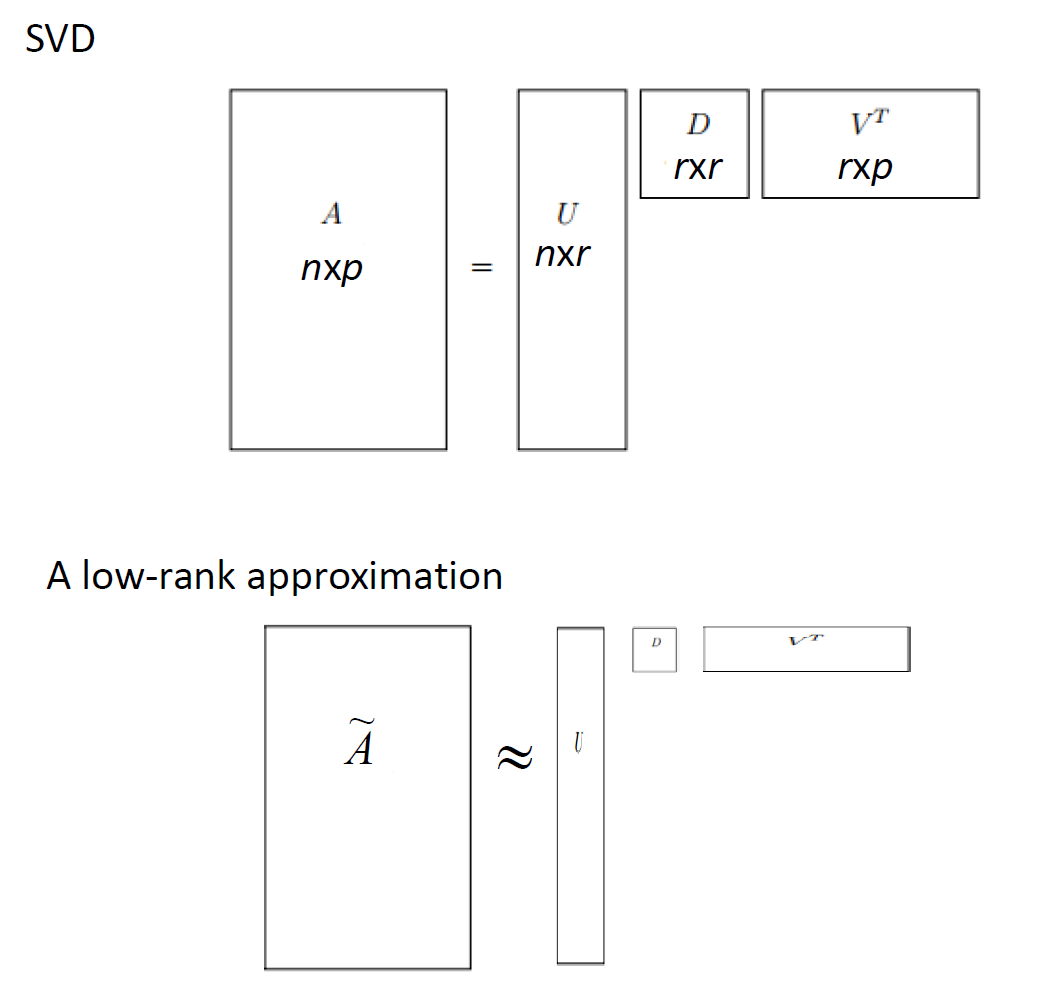
\includegraphics[width=0.6\linewidth]{img/SVD_Approx}
\end{frame}

\begin{frame}{SVD: Example 1}
\protect\hypertarget{svd-example-1}{}
*The original image

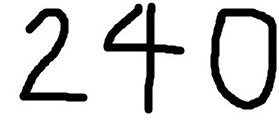
\includegraphics[width=0.6\linewidth]{img/svdexample}
\end{frame}

\begin{frame}{SVD: Example 1}
\protect\hypertarget{svd-example-1-1}{}
*The original image

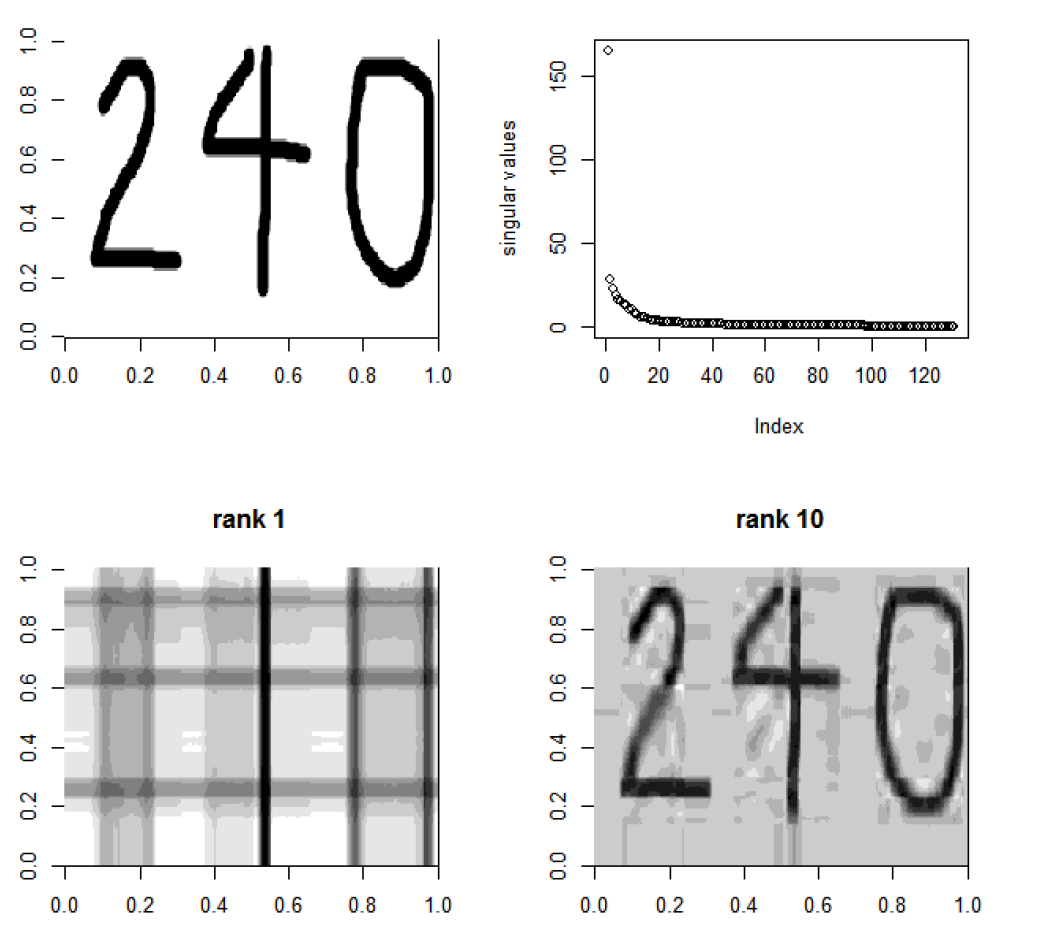
\includegraphics[width=0.6\linewidth]{img/240svd_Approx}
\end{frame}

\begin{frame}[fragile]{SVD: Example 1}
\protect\hypertarget{svd-example-1-2}{}
\begin{Shaded}
\begin{Highlighting}[]
\CommentTok{\#install and load "jpeg"}
\FunctionTok{library}\NormalTok{(jpeg)}
\NormalTok{mydata}\OtherTok{=}\FunctionTok{readJPEG}\NormalTok{(}\StringTok{"img/svdexample.jpg"}\NormalTok{, }\AttributeTok{native =} \ConstantTok{FALSE}\NormalTok{)}
\NormalTok{mydata}\OtherTok{=}\NormalTok{mydata[,,}\DecValTok{1}\NormalTok{] }\CommentTok{\#279{-}by{-}131}
\NormalTok{obj}\OtherTok{=}\FunctionTok{svd}\NormalTok{(mydata)}
\CommentTok{\#obj$u: a 279{-}by{-}131 matrix}
\CommentTok{\#obj$d: a vector of 131 nonnegative values}
\CommentTok{\#obj$v: a 131{-}by{-}131 matrix}
\end{Highlighting}
\end{Shaded}
\end{frame}

\begin{frame}[fragile]{SVD Example 1: R}
\protect\hypertarget{svd-example-1-r}{}
\begin{Shaded}
\begin{Highlighting}[]
\FunctionTok{par}\NormalTok{(}\AttributeTok{mfrow=}\FunctionTok{c}\NormalTok{(}\DecValTok{2}\NormalTok{,}\DecValTok{2}\NormalTok{))}
\FunctionTok{image}\NormalTok{(mydata,}\AttributeTok{col=}\FunctionTok{gray}\NormalTok{(}\FunctionTok{c}\NormalTok{(}\DecValTok{0}\SpecialCharTok{:}\DecValTok{10}\NormalTok{)}\SpecialCharTok{/}\DecValTok{10}\NormalTok{))}

\FunctionTok{plot}\NormalTok{(obj}\SpecialCharTok{$}\NormalTok{d, }\AttributeTok{ylab=}\StringTok{"singular values"}\NormalTok{)}

\NormalTok{n}\OtherTok{=}\DecValTok{1}
\NormalTok{mydata.approx}\OtherTok{=}\NormalTok{obj}\SpecialCharTok{$}\NormalTok{u[,}\DecValTok{1}\NormalTok{] }\SpecialCharTok{\%*\%} \FunctionTok{t}\NormalTok{(obj}\SpecialCharTok{$}\NormalTok{v[,}\DecValTok{1}\NormalTok{])}\SpecialCharTok{*}\NormalTok{obj}\SpecialCharTok{$}\NormalTok{d[}\DecValTok{1}\NormalTok{]}
\FunctionTok{image}\NormalTok{(mydata.approx, }\AttributeTok{main=}\StringTok{"rank 1"}\NormalTok{, }\AttributeTok{col=}\FunctionTok{gray}\NormalTok{(}\FunctionTok{c}\NormalTok{(}\DecValTok{0}\SpecialCharTok{:}\DecValTok{10}\NormalTok{)}\SpecialCharTok{/}\DecValTok{10}\NormalTok{))}

\NormalTok{n}\OtherTok{=}\DecValTok{10}
\NormalTok{mydata.approx}\OtherTok{=}\NormalTok{obj}\SpecialCharTok{$}\NormalTok{u[,}\DecValTok{1}\SpecialCharTok{:}\NormalTok{n]}\SpecialCharTok{\%*\%} \FunctionTok{diag}\NormalTok{(obj}\SpecialCharTok{$}\NormalTok{d[}\DecValTok{1}\SpecialCharTok{:}\NormalTok{n]) }\SpecialCharTok{\%*\%} \FunctionTok{t}\NormalTok{(obj}\SpecialCharTok{$}\NormalTok{v[,}\DecValTok{1}\SpecialCharTok{:}\NormalTok{n])}
\FunctionTok{image}\NormalTok{(mydata.approx, }\AttributeTok{main=}\StringTok{"rank 10"}\NormalTok{, }\AttributeTok{col=}\FunctionTok{gray}\NormalTok{(}\FunctionTok{c}\NormalTok{(}\DecValTok{0}\SpecialCharTok{:}\DecValTok{10}\NormalTok{)}\SpecialCharTok{/}\DecValTok{10}\NormalTok{))}
\end{Highlighting}
\end{Shaded}
\end{frame}

\begin{frame}{SVD Example 1: R}
\protect\hypertarget{svd-example-1-r-1}{}
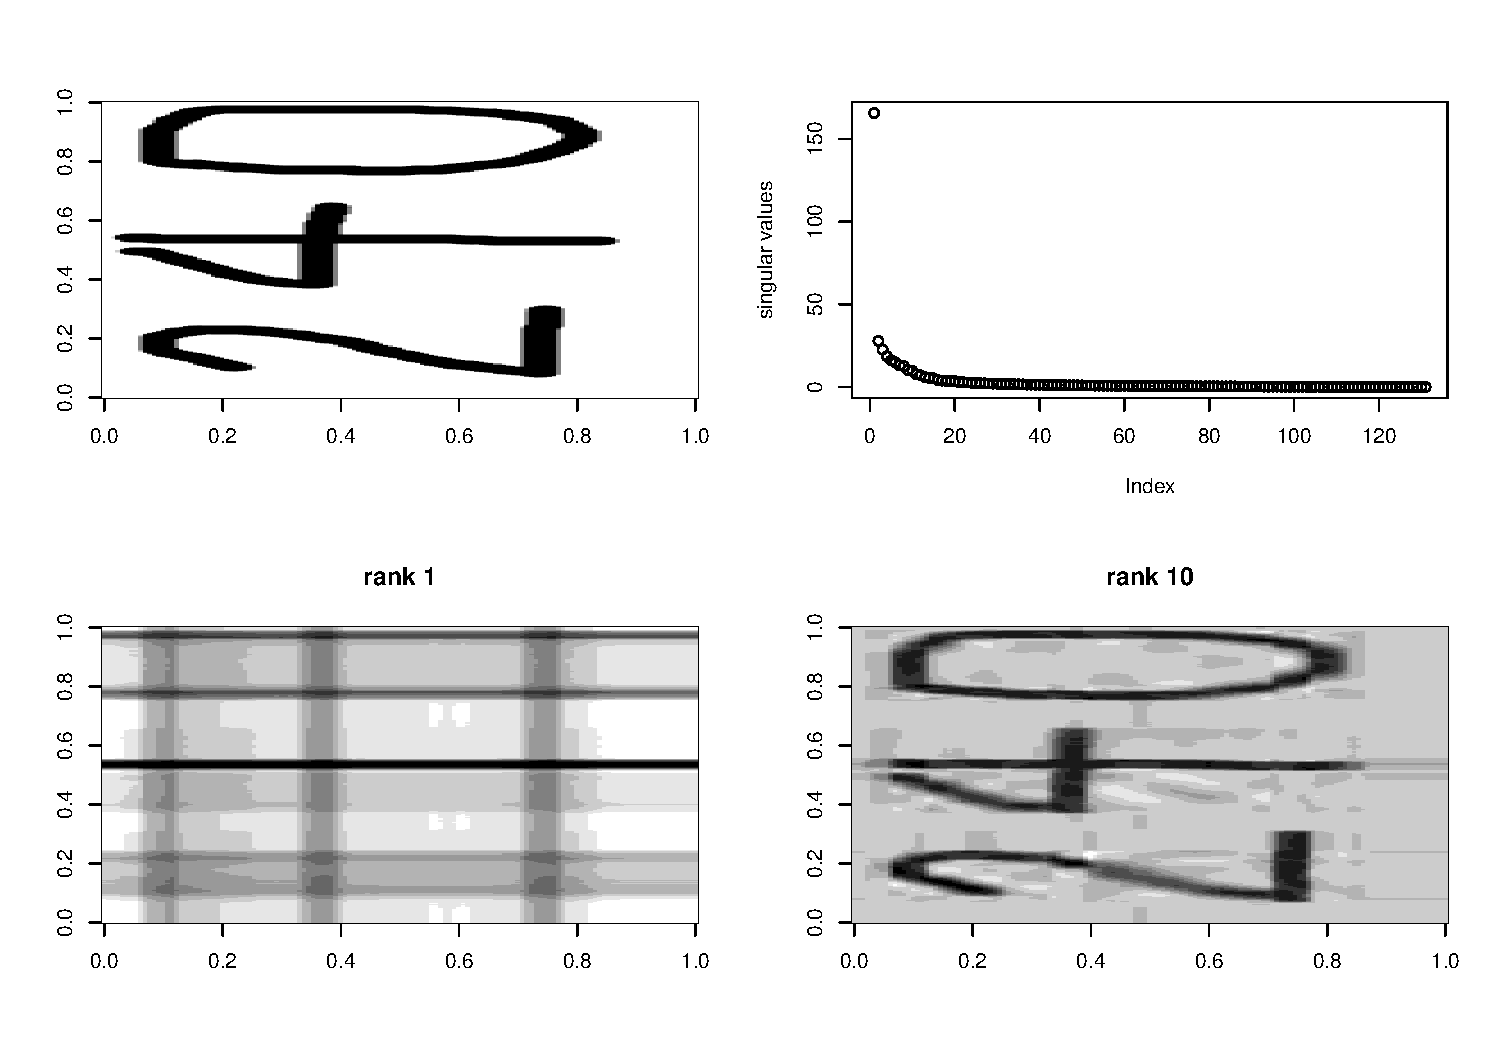
\includegraphics{Lecture02_MatrixOperations_files/figure-beamer/unnamed-chunk-21-1.pdf}
\end{frame}

\begin{frame}[fragile]{SVD: Example 2}
\protect\hypertarget{svd-example-2}{}
\begin{Shaded}
\begin{Highlighting}[]
\NormalTok{BikeMan}\OtherTok{=}\FunctionTok{readJPEG}\NormalTok{(}\StringTok{"BikeMan.jpg"}\NormalTok{, }\AttributeTok{native =} \ConstantTok{FALSE}\NormalTok{)}
\NormalTok{BikeMan}\OtherTok{=}\NormalTok{BikeMan[,,}\DecValTok{1}\NormalTok{]}

\FunctionTok{par}\NormalTok{(}\AttributeTok{mfrow=}\FunctionTok{c}\NormalTok{(}\DecValTok{2}\NormalTok{,}\DecValTok{2}\NormalTok{))}
\FunctionTok{image}\NormalTok{(BikeMan, }\AttributeTok{col=}\FunctionTok{gray}\NormalTok{(}\FunctionTok{c}\NormalTok{(}\DecValTok{0}\SpecialCharTok{:}\DecValTok{10}\NormalTok{)}\SpecialCharTok{/}\DecValTok{10}\NormalTok{))}
\NormalTok{obj.bm}\OtherTok{=}\FunctionTok{svd}\NormalTok{(BikeMan)}

\NormalTok{n}\OtherTok{=}\DecValTok{10}
\NormalTok{BikeMan.approx}\OtherTok{=}\NormalTok{obj.bm}\SpecialCharTok{$}\NormalTok{u[,}\DecValTok{1}\SpecialCharTok{:}\NormalTok{n]}\SpecialCharTok{\%*\%} \FunctionTok{diag}\NormalTok{(obj.bm}\SpecialCharTok{$}\NormalTok{d[}\DecValTok{1}\SpecialCharTok{:}\NormalTok{n]) }\SpecialCharTok{\%*\%} \FunctionTok{t}\NormalTok{(obj.bm}\SpecialCharTok{$}\NormalTok{v[,}\DecValTok{1}\SpecialCharTok{:}\NormalTok{n])}
\FunctionTok{image}\NormalTok{(BikeMan.approx, }\AttributeTok{main=}\StringTok{"rank 10"}\NormalTok{, }\AttributeTok{col=}\FunctionTok{gray}\NormalTok{(}\FunctionTok{c}\NormalTok{(}\DecValTok{0}\SpecialCharTok{:}\DecValTok{10}\NormalTok{)}\SpecialCharTok{/}\DecValTok{10}\NormalTok{))}

\NormalTok{n}\OtherTok{=}\DecValTok{20}
\NormalTok{BikeMan.approx}\OtherTok{=}\NormalTok{obj.bm}\SpecialCharTok{$}\NormalTok{u[,}\DecValTok{1}\SpecialCharTok{:}\NormalTok{n]}\SpecialCharTok{\%*\%} \FunctionTok{diag}\NormalTok{(obj.bm}\SpecialCharTok{$}\NormalTok{d[}\DecValTok{1}\SpecialCharTok{:}\NormalTok{n]) }\SpecialCharTok{\%*\%} \FunctionTok{t}\NormalTok{(obj.bm}\SpecialCharTok{$}\NormalTok{v[,}\DecValTok{1}\SpecialCharTok{:}\NormalTok{n])}
\FunctionTok{image}\NormalTok{(BikeMan.approx, }\AttributeTok{main=}\StringTok{"rank 20"}\NormalTok{, }\AttributeTok{col=}\FunctionTok{gray}\NormalTok{(}\FunctionTok{c}\NormalTok{(}\DecValTok{0}\SpecialCharTok{:}\DecValTok{10}\NormalTok{)}\SpecialCharTok{/}\DecValTok{10}\NormalTok{))}

\NormalTok{n}\OtherTok{=}\DecValTok{30}
\NormalTok{BikeMan.approx}\OtherTok{=}\NormalTok{obj.bm}\SpecialCharTok{$}\NormalTok{u[,}\DecValTok{1}\SpecialCharTok{:}\NormalTok{n]}\SpecialCharTok{\%*\%} \FunctionTok{diag}\NormalTok{(obj.bm}\SpecialCharTok{$}\NormalTok{d[}\DecValTok{1}\SpecialCharTok{:}\NormalTok{n]) }\SpecialCharTok{\%*\%} \FunctionTok{t}\NormalTok{(obj.bm}\SpecialCharTok{$}\NormalTok{v[,}\DecValTok{1}\SpecialCharTok{:}\NormalTok{n])}
\FunctionTok{image}\NormalTok{(BikeMan.approx, }\AttributeTok{main=}\StringTok{"rank 30"}\NormalTok{, }\AttributeTok{col=}\FunctionTok{gray}\NormalTok{(}\FunctionTok{c}\NormalTok{(}\DecValTok{0}\SpecialCharTok{:}\DecValTok{10}\NormalTok{)}\SpecialCharTok{/}\DecValTok{10}\NormalTok{))}
\end{Highlighting}
\end{Shaded}
\end{frame}

\begin{frame}{SVD: Example 2}
\protect\hypertarget{svd-example-2-1}{}
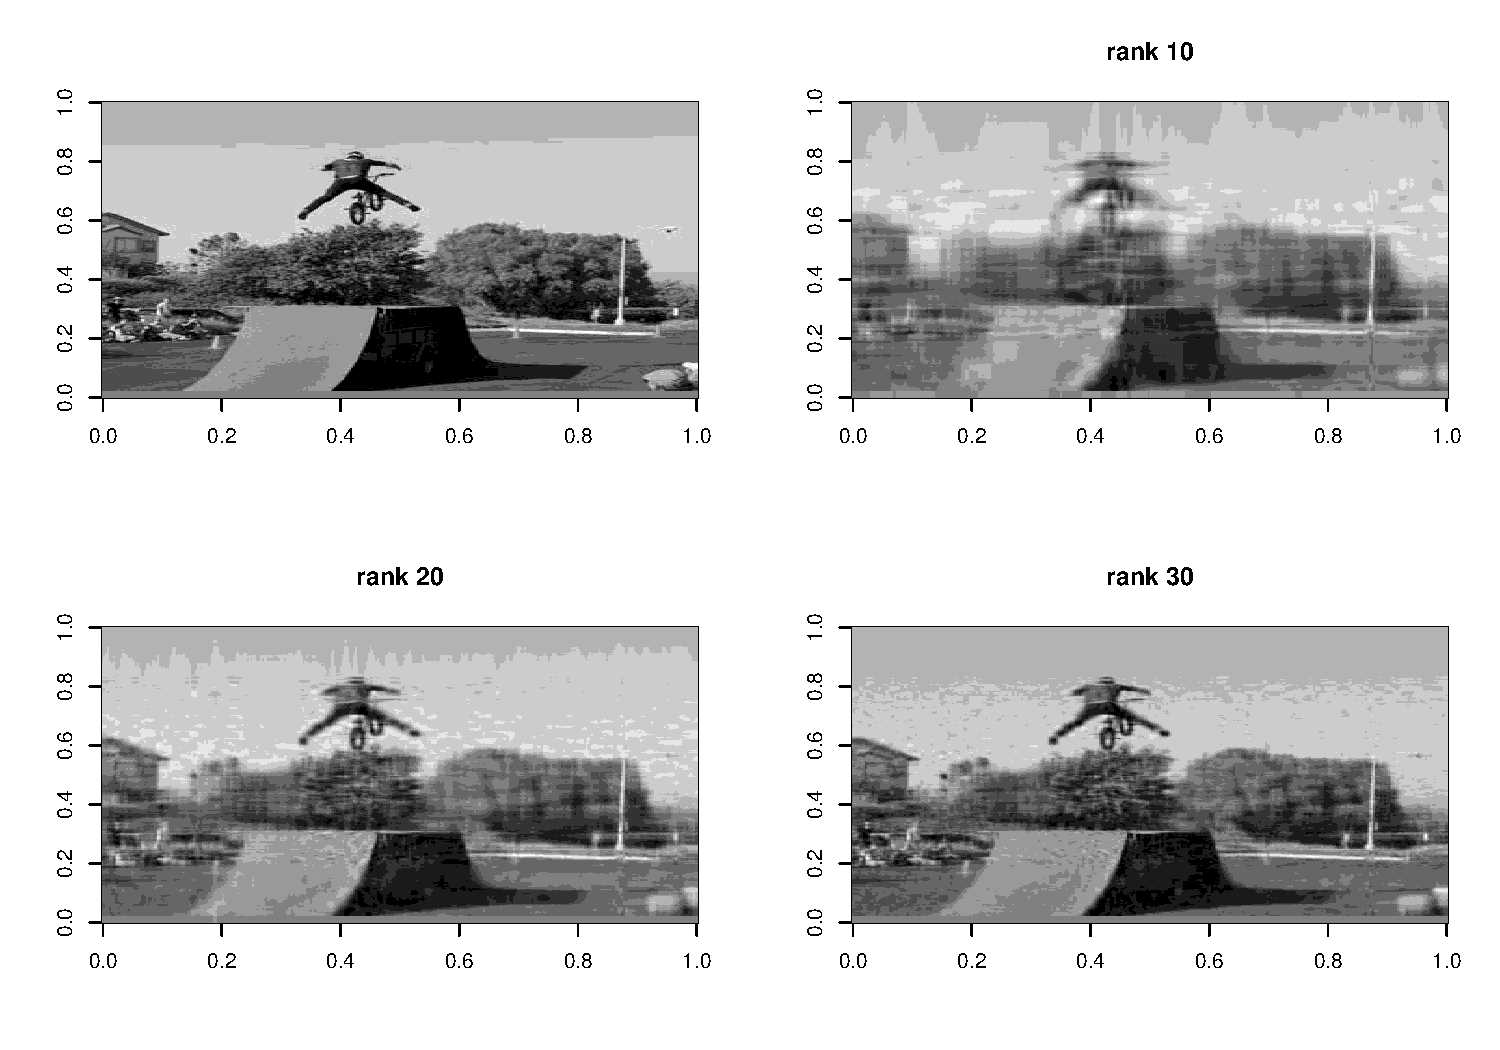
\includegraphics{Lecture02_MatrixOperations_files/figure-beamer/unnamed-chunk-23-1.pdf}
\end{frame}

\hypertarget{another-matrix-operation-kronecker-product}{%
\subsection{Another Matrix Operation: Kronecker
Product}\label{another-matrix-operation-kronecker-product}}

\begin{frame}{Definition}
\protect\hypertarget{definition}{}
\begin{itemize}
\tightlist
\item
  The Kronecker product, denoted by \(\bigotimes\) is a mathematical
  operation that combines two matrices to create a larger matrix.
\item
  \textcolor{pink}{It is named after the Danish mathematician Heinrich Kronecker, who introduced it in the late 19th century.}
  Chatgpt gives \textcolor{red}{wrong} information.
\item
  According to wikipedia, ``The Kronecker product is named after the
  German mathematician Leopold Kronecker (1823--1891), even though there
  is little evidence that he was the first to define and use it.''
\item
  Why is it useful? It provide compact Representation. Kronecker product
  allows for compact representation of large matrices by expressing them
  as a combination of smaller matrices.
\end{itemize}
\end{frame}

\begin{frame}{Definition}
\protect\hypertarget{definition-1}{}
Let \[A_{m\times n}=\begin{pmatrix}
a_{11} & \cdots & a_{1n}\\
\cdots & \cdots & \cdots\\
a_{m1} & \cdots & a_{mn}\\
\end{pmatrix},
B_{p\times q}=\begin{pmatrix}
b_{11} & \cdots & b_{1q}\\
\cdots & \cdots & \cdots\\
b_{p1} & \cdots & b_{pq}\\
\end{pmatrix}\] Then, \[A \bigotimes B = 
\begin{pmatrix}
a_{11} * B & a_{12} * B & ... & a_{1n} * B \\
\cdots & \cdots & \cdots & \cdots\\
a_{m1} * B & a_{m2} * B & ... & a_{mn} * B 
\end{pmatrix}\]
\end{frame}

\begin{frame}{Definition}
\protect\hypertarget{definition-2}{}
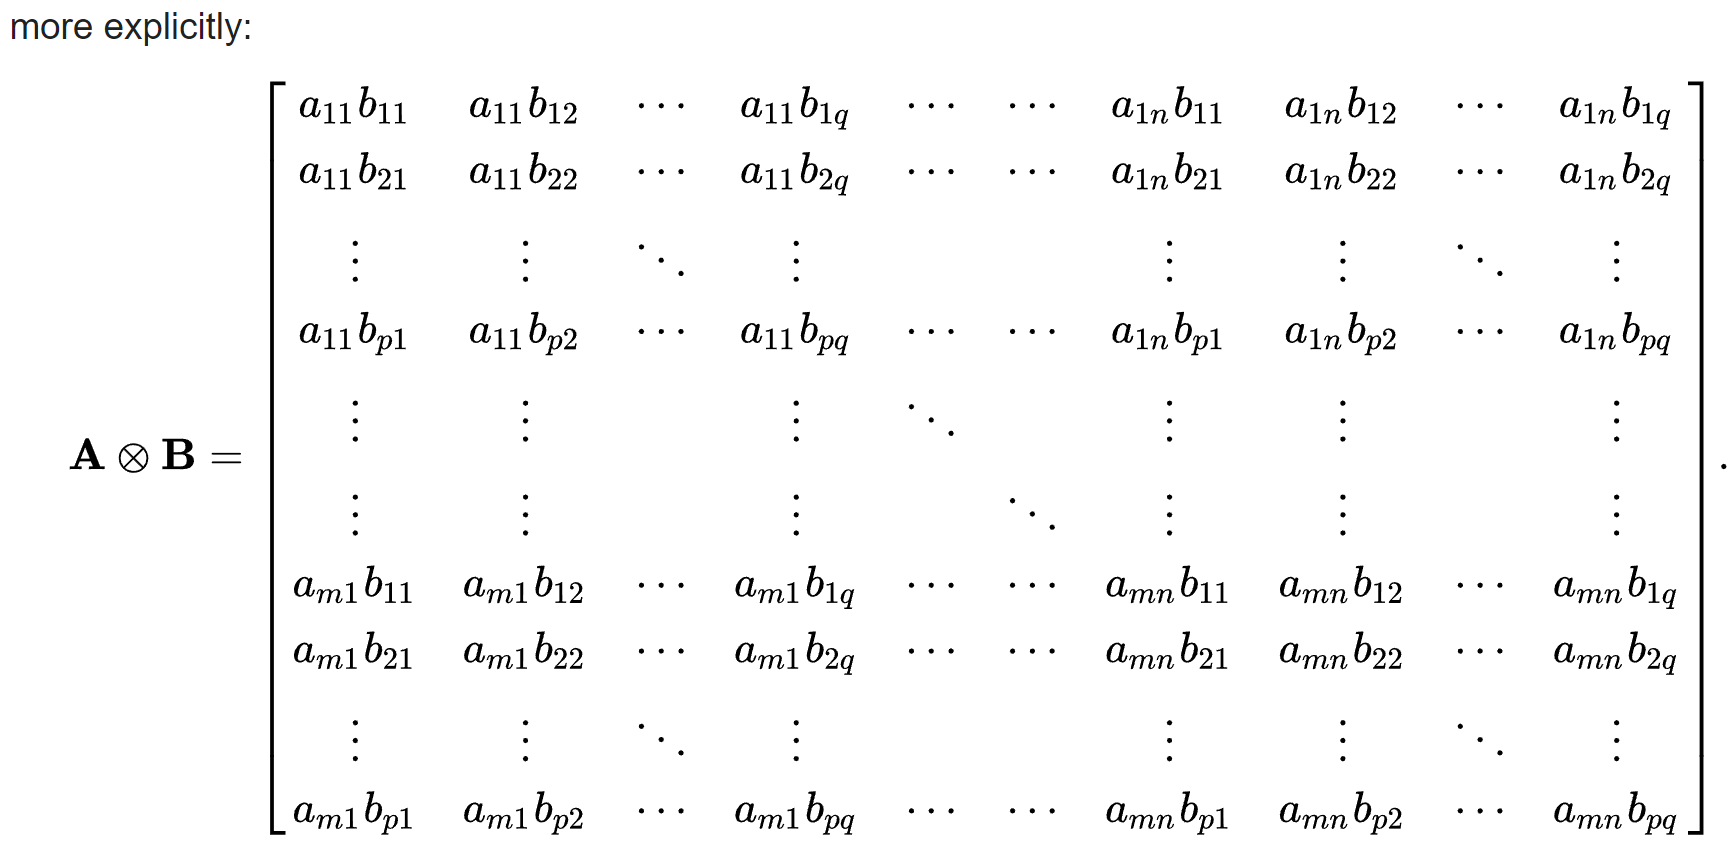
\includegraphics[width=0.8\linewidth]{img/kronecker_prod}
\end{frame}

\hypertarget{futher-reading}{%
\subsection{Futher reading}\label{futher-reading}}

\begin{frame}{Futher reading}
\begin{itemize}
\tightlist
\item
  Chronecker product: Gerald S. Rogers. (1984) Kronecker Products in
  ANOVA-A First Step. The American Statistician, 38: 197-202.
\item
  SVD: Biclustering via Sparse Singular Value Decomposition''
  \url{https://www.unc.edu/~haipeng/publication/ssvd.pdf}
\end{itemize}
\end{frame}

\hypertarget{homework-1-due-on}{%
\subsection{\texorpdfstring{Homework 1 (Due on
\textcolor{red}{April 2023})}{Homework 1 (Due on )}}\label{homework-1-due-on}}

\begin{frame}{Problem 1}
\protect\hypertarget{problem-1}{}
\begin{itemize}
\tightlist
\item
  Suppose \(X_1, X_2, Y_1, Y_2\) are mutually independent.

  \begin{itemize}
  \tightlist
  \item
    \(X_1\) and \(X_2\) are iid from \(N(\mu=0, \sigma_x^2=2^2)\)
  \item
    \(Y_1\) and \(Y_2\) are iid from \(N(\mu=0, \sigma_y^2=1^2)\)
    Consider the two pairs \((X_1, X_2)\) and \((Y_1, Y_2)\). Which pair
    tends to have a larger difference? To answer the question, please
    calculate and estimate the following two probabilities:
    \[P(|X_1-X_2|>4), P(|Y_1-Y_2|>4)\]
  \end{itemize}
\item
  The hints for calculating/estimating \(P(|X_1-X_2|>4)\) can be found
  in the two slides. Using similar strategies, you can
  calculate/estimate \(P(|Y_1-Y_2|>4)\)
\end{itemize}
\end{frame}

\begin{frame}{Calculate \(P(|X_1-X_2|>4)\)}
\protect\hypertarget{calculate-px_1-x_24}{}
\begin{itemize}
\tightlist
\item
  Hints for calculating \(P(|X_1-X_2|>4)\).

  \begin{itemize}
  \tightlist
  \item
    First find the distribution of \(X_1-X_2\). Then standard it to have
    mean 0 and SD 1.
  \item
    Second, express the probability to \(P(|Z|>z)\), where
    \(Z\sim N(0,1)\).
  \item
    Next, expression the probability in terms of \(\Phi(\cdot)\), the
    CDF of the standard normal distribution.
  \item
    Last, use the ``pnorm'' function in R to find the numerical value.
  \end{itemize}
\end{itemize}
\end{frame}

\begin{frame}{Estimate \(P(|X_1-X_2|>4)\)}
\protect\hypertarget{estimate-px_1-x_24}{}
\begin{itemize}
\tightlist
\item
  The probability can be estimated by doing simulations/sampling.
\item
  If you sample many (say 10,000) pairs of \(X_1\) and \(X_2\), count
  how many pairs satisfying \(|X_1-X_2|>4\). The probability can be used
  to estimate \(P(|X_1-X_2|>4)\)
\end{itemize}
\end{frame}

\begin{frame}[fragile]{Problem 2}
\protect\hypertarget{problem-2}{}
\begin{itemize}
\tightlist
\item
  Find a matrix \(A\) such that \(AY\) gives the difference of means
  vectors between iris setosa and iris versicolor
\item
  Find a matrix \(B\) such that \(YB\) is column-standardized, i.e., the
  standard deviation of each column/feature is 1.
\item
  Check the following

  \begin{itemize}
  \tightlist
  \item
    Let \(C=\mathbf I_{150} - \frac{1}{150}J\), where
    \(J_{150\times 150}\) is an all-ones matrices . Use R to verify that
    \(CY\) centers each column/feature. The R code for \(C\) is ''
  \end{itemize}

\begin{verbatim}
C=diag(1,150) - \frac{150}matrix(1, 150, 150)
\end{verbatim}

  \begin{itemize}
  \tightlist
  \item
    Let \(S\) be the sample covariance matrix. Use R to verify that each
    column of \(CYS^{-1/2}\) has been centered and standardized. Hints:
  \end{itemize}

\begin{verbatim}
S=cov(Y)
\end{verbatim}

  To compute \(S^{-1/2}\), you may need a R package, such as
  ``qtl2pleio''.
\end{itemize}
\end{frame}

\begin{frame}{Problem 3}
\protect\hypertarget{problem-3}{}
\begin{itemize}
\tightlist
\item
  Choose a picture you like and conduct approximations using singular
  value decomposition (SVD).
\end{itemize}
\end{frame}

\end{document}
